\documentclass[25pt, a0paper, landscape, margin=0mm, innermargin=14mm, blockverticalspace=12mm, colspace=14mm]{tikzposter}
\usepackage{booktabs}
\usepackage{graphicx}
\usepackage{xcolor}
\usetikzlibrary{arrows.meta, positioning, calc}

\definecolor{ink}{HTML}{0B0B0B}
\definecolor{ink2}{HTML}{52514E}
\definecolor{surface}{HTML}{FCFCFB}
\definecolor{accent}{HTML}{2A78D6}
\definecolor{ours}{HTML}{E87BA4}
\definecolor{good}{HTML}{006300}
\definecolor{bad}{HTML}{D03B3B}
\definecolor{rule}{HTML}{E1E0D9}

\definecolorstyle{clean}{
  \definecolor{colorOne}{HTML}{0B0B0B}
  \definecolor{colorTwo}{HTML}{2A78D6}
  \definecolor{colorThree}{HTML}{FCFCFB}
}{
  \colorlet{backgroundcolor}{colorThree}
  \colorlet{framecolor}{colorThree}
  \colorlet{titlefgcolor}{colorOne}
  \colorlet{titlebgcolor}{colorThree}
  \colorlet{blocktitlebgcolor}{colorThree}
  \colorlet{blocktitlefgcolor}{colorTwo}
  \colorlet{blockbodybgcolor}{colorThree}
  \colorlet{blockbodyfgcolor}{colorOne}
  \colorlet{innerblocktitlebgcolor}{colorThree}
  \colorlet{innerblocktitlefgcolor}{colorOne}
  \colorlet{innerblockbodybgcolor}{colorThree}
  \colorlet{innerblockbodyfgcolor}{colorOne}
  \colorlet{notefgcolor}{colorOne}
  \colorlet{notebgcolor}{colorThree}
  \colorlet{notefrcolor}{colorThree}
}
\usecolorstyle{clean}
\defineblockstyle{lined}{titlewidthscale=1, bodywidthscale=1, titleleft, titleoffsetx=0pt, titleoffsety=0pt,
  bodyoffsetx=0pt, bodyoffsety=0pt, bodyverticalshift=0pt, roundedcorners=0, linewidth=0pt, titleinnersep=6mm,
  bodyinnersep=6mm}{
  \draw[draw=rule, line width=1.2mm] ([yshift=0mm]blocktitle.north west) -- ([yshift=0mm]blocktitle.north east);
}
\useblockstyle{lined}
\usetitlestyle{Empty}

\title{\parbox{0.9\linewidth}{\centering Beyond Remembering: Maintaining Active Constraints and Pending Commitments Across Context Compaction}}
\author{Sheng Lu \quad Qixiang Fan \quad Ziyan Fan \quad Xiuping Zhu}
\institute{Georgia Institute of Technology \quad\textbullet\quad ECE 6256 / CS 6604, Fall 2026}

\newcommand{\hero}[1]{{\fontsize{60}{66}\selectfont\bfseries #1}}
\newcommand{\st}[1]{\texttt{#1}}

\begin{document}
\maketitle[titletotopverticalspace=20mm, titletoblockverticalspace=16mm]

\begin{columns}
%% ------------------------------------------------------------ column 1
\column{0.3}
\block{The problem: memory is not just recall}{
An agent must know what it is \textbf{still} allowed or obliged to do:

\vspace{4mm}
\begin{tabular}{@{}ll@{}}
\textit{``Don't send the report until I approve the final version.''} & \\[2mm]
\quad$\rightarrow$ approval of the \textit{outline} & \textcolor{bad}{still wait} \\
\quad$\rightarrow$ approval of the \textit{final version} & \textcolor{good}{act} \\
\quad$\rightarrow$ tool receipt: \st{SUCCESS} & \textcolor{bad}{never send again} \\
\end{tabular}

\vspace{6mm}
Context \textbf{compaction} replaces old turns with a summary. Prior work: compaction drops \emph{static} constraints. We study state that \textbf{changes after it is stated}: revoked prohibitions, triggered and discharged commitments.

\vspace{4mm}
\textbf{RQ1} Does mutable state go \emph{stale} rather than \emph{missing}?\\
\textbf{RQ2} At equal memory budget, does lifecycle tracking beat pinning and chronological memory?\\
\textbf{RQ3} Bad stored state, or bad decisions given correct state?
}

\block{Lifecycle-Aware Dialogue Ledger (LADL)}{
\centering
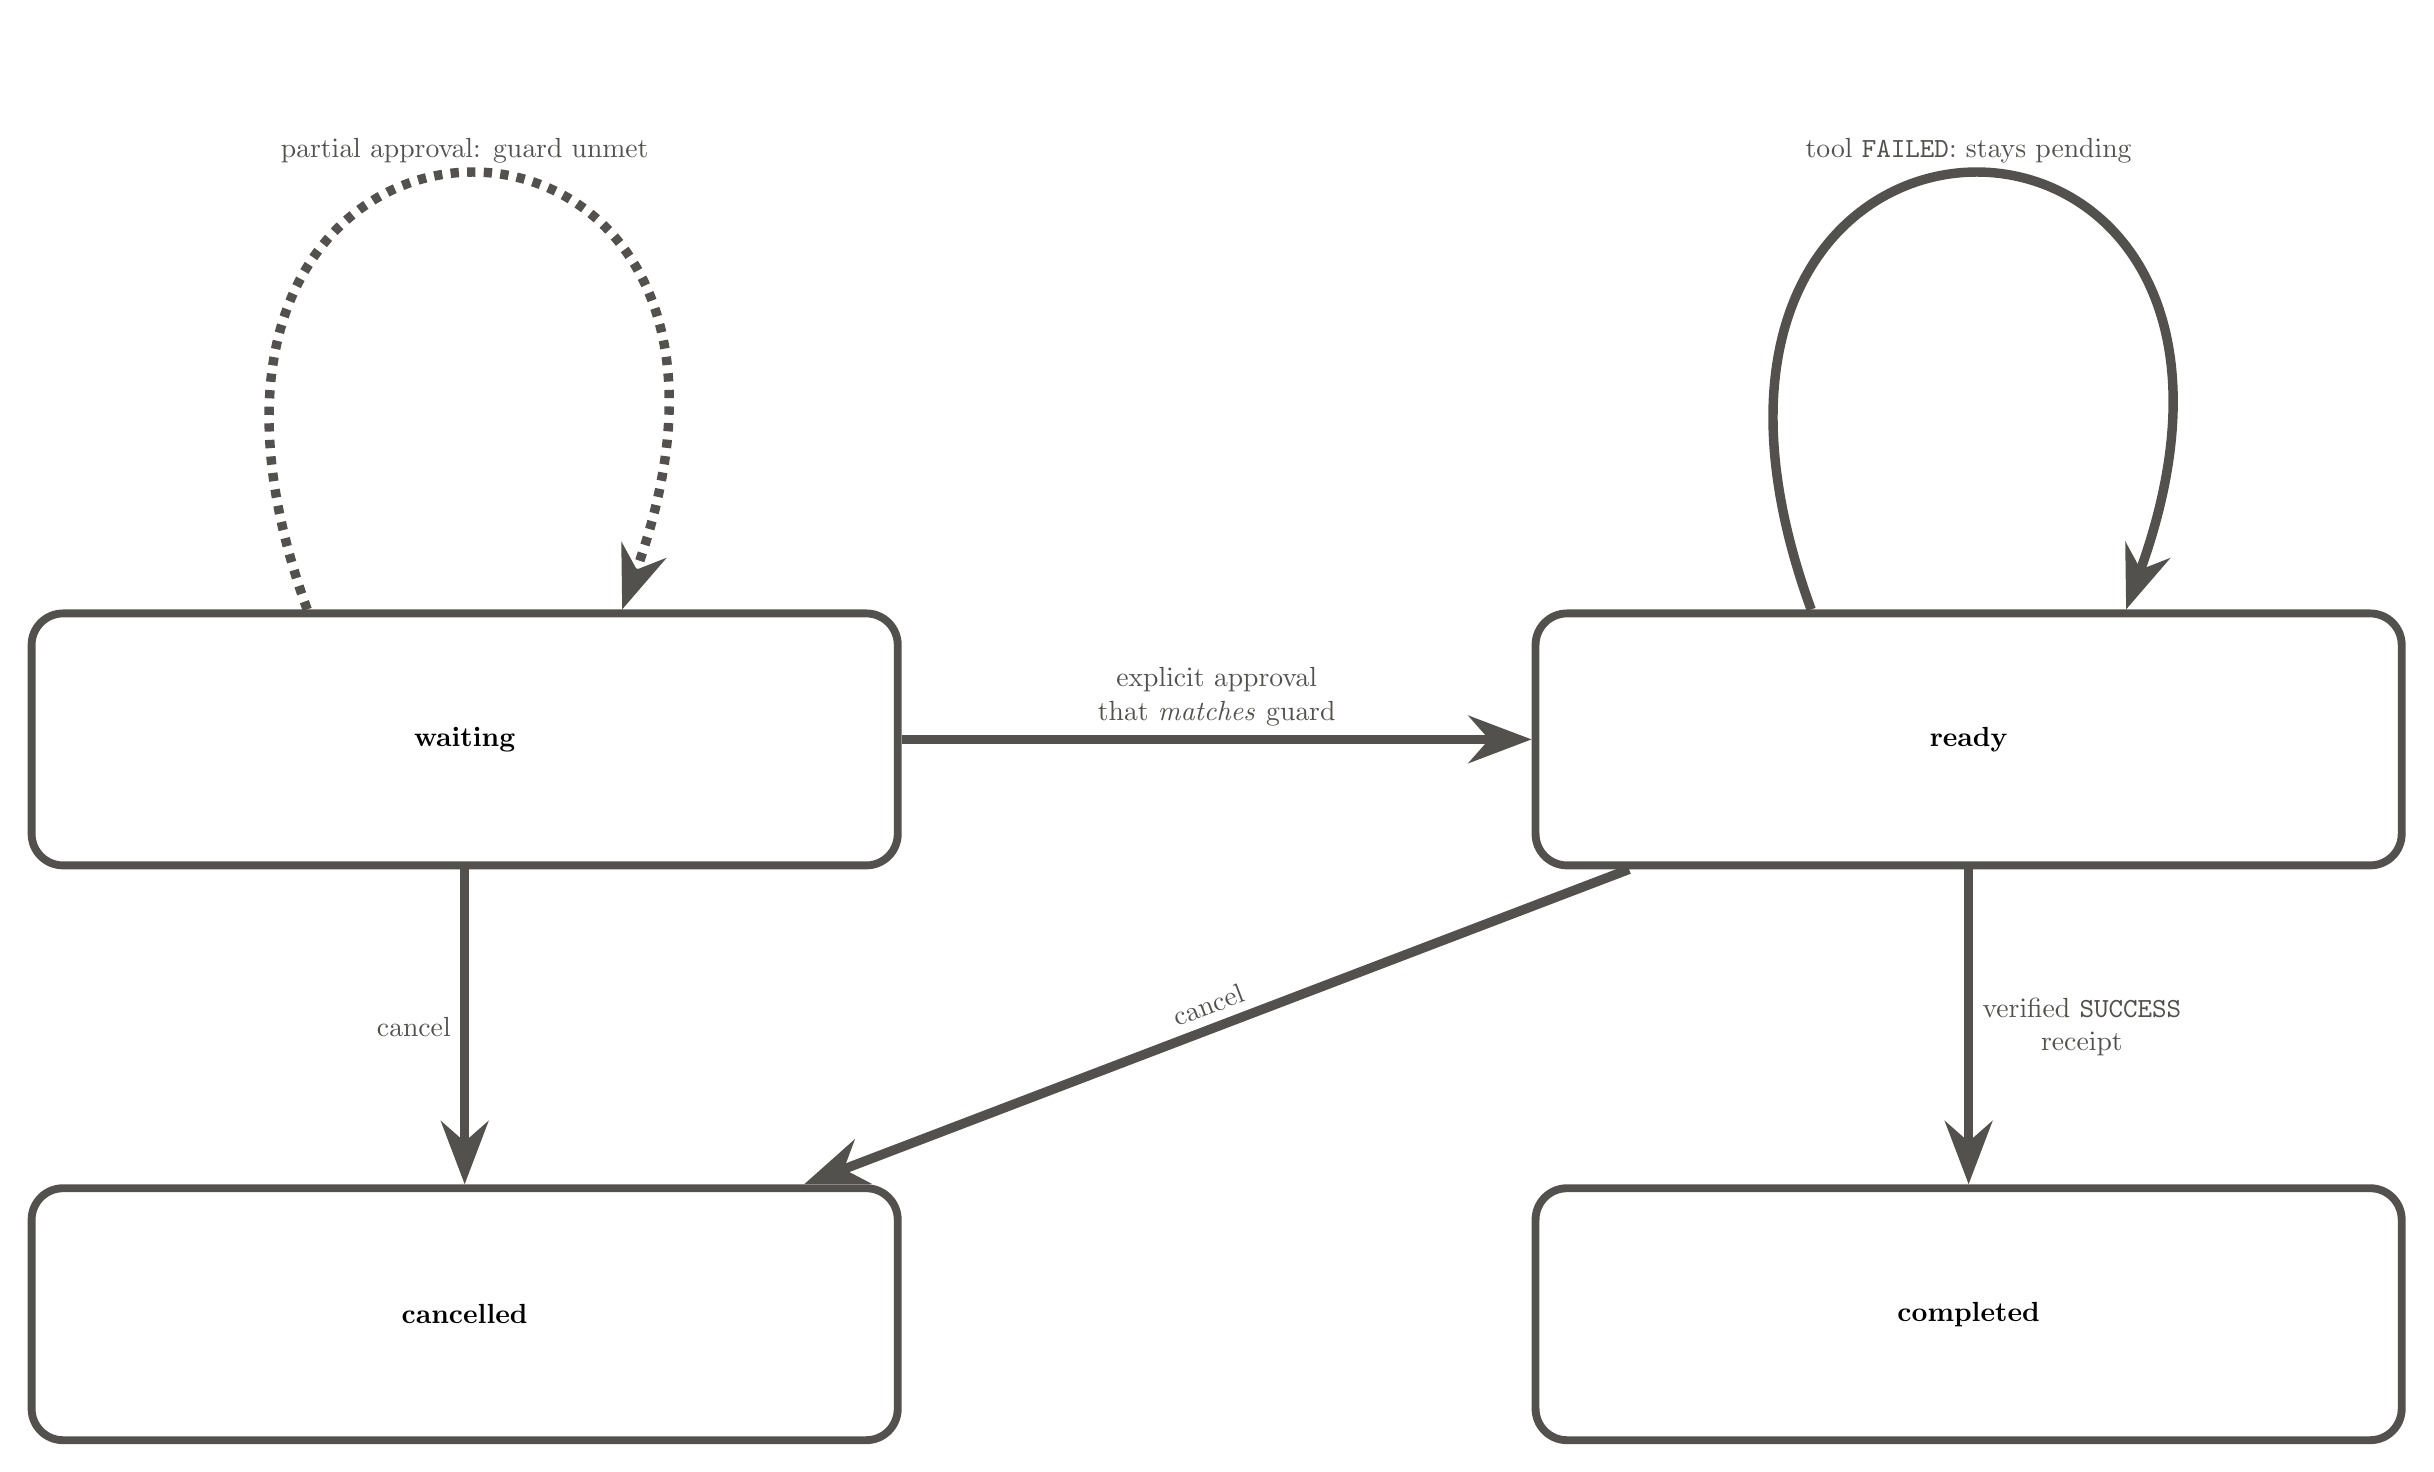
\begin{tikzpicture}[st/.style={draw=ink2, rounded corners=4mm, line width=1mm, minimum width=11cm, minimum height=3.2cm, font=\bfseries},
  ar/.style={-{Stealth[length=8mm]}, line width=1.2mm, draw=ink2}, lab/.style={font=\normalsize, text=ink2, align=center}]
  \node[st] (w) {waiting};
  \node[st, right=8cm of w] (r) {ready};
  \node[st, below=4cm of r] (c) {completed};
  \node[st, below=4cm of w] (x) {cancelled};
  \draw[ar] (w) -- node[lab, above] {explicit approval\\that \emph{matches} guard} (r);
  \draw[ar] (r) -- node[lab, right] {verified \st{SUCCESS}\\receipt} (c);
  \draw[ar] (r.north) ++(-2cm,0) to[out=110, in=70, looseness=5] node[lab, above] {tool \st{FAILED}: stays pending} ($(r.north)+(2cm,0)$);
  \draw[ar] (w) -- node[lab, left] {cancel} (x);
  \draw[ar] (r) -- node[lab, sloped, above] {cancel} (x);
  \draw[ar, dashed] (w.north) ++(-2cm,0) to[out=110, in=70, looseness=5] node[lab, above] {partial approval: guard unmet} ($(w.north)+(2cm,0)$);
\end{tikzpicture}

\vspace{4mm}
\raggedright
Prohibitions: \st{active} $\leftrightarrow$ \st{revoked}. Hedged updates set an \emph{unclear} flag $\Rightarrow$ ask.
\begin{itemize}
\item An LLM \textbf{extracts} typed events per turn; a \textbf{deterministic reducer} applies the transitions, each logged with its evidence turn.
\item At each compaction, the dialogue becomes a summary; the \textbf{current-state ledger persists} beside it within the same token budget.
\item The policy chooses \st{act} / \st{wait} / \st{clarify} / \st{decline}.
\end{itemize}
}

%% ------------------------------------------------------------ column 2
\column{0.4}
\block{Benchmark}{
48 hand-designed gold event timelines (13 families: revocation, completion + repeat request, conditional triggering incl. misleading partial approvals, plus a static control) $\rightarrow$ \textbf{192 dialogues}, 24--42 turns, \textbf{1--5 compactions}, \textbf{872 decision probes} with programmatic gold states and permissible actions. Held-out templates for test (664 probes); LLM paraphrases checked by an equivalence judge + manual audit (38/40 OK).
}

\block{RQ2: action accuracy at a matched 384-token budget}{
\centering
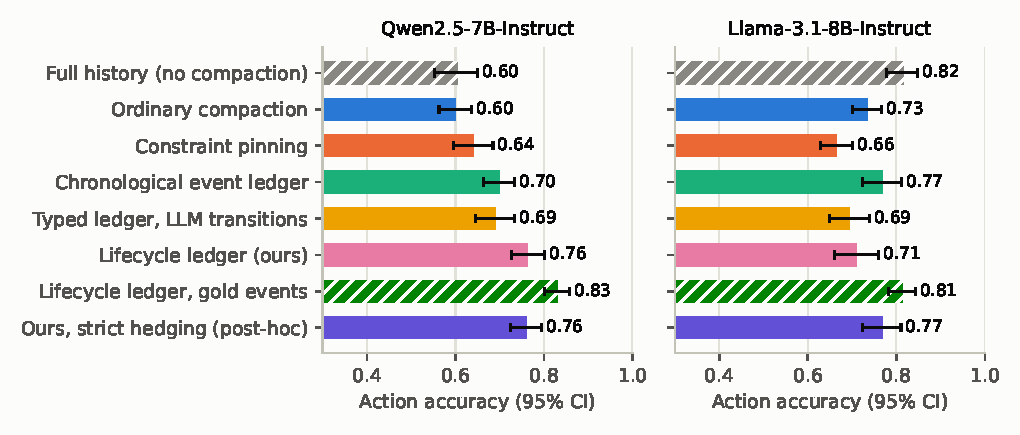
\includegraphics[width=0.97\linewidth]{../results/figures/fig_main_accuracy.pdf}

\vspace{4mm}
\raggedright
\begin{itemize}
\item \textbf{Qwen2.5-7B:} LADL \hero{76.4\%} vs.\ ordinary compaction 60.1\% (+16.3 pp), pinning 64.2\% (+12.2), chronological ledger 69.9\% (+6.5), LLM transitions 69.1\% (+7.2); all $p\le0.002$ (timeline-clustered bootstrap). Violations 12.5\% $\rightarrow$ 4.7\%.
\item \textbf{Llama-3.1-8B:} no gain (71.1\% vs.\ 73.5\%), yet the \emph{gold-event} ledger reaches 81.5\% $\Rightarrow$ the bottleneck is extraction (see RQ3).
\end{itemize}
}

\block{Accuracy decays with each compaction since the item last changed}{
\centering
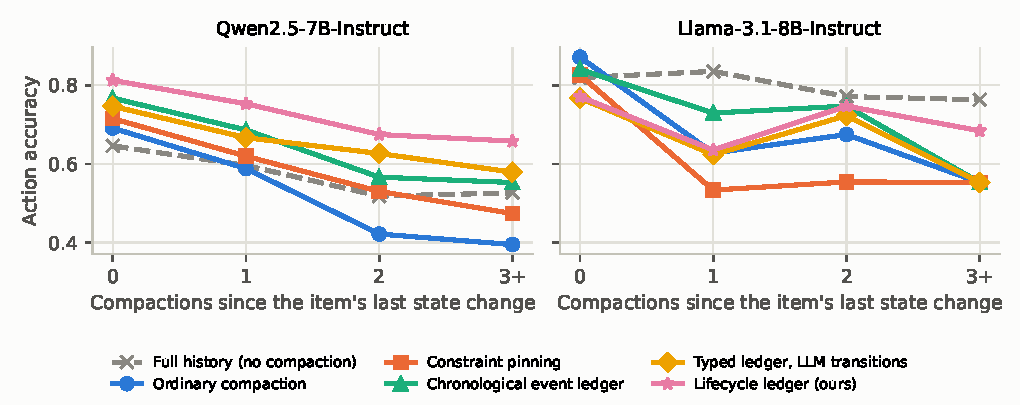
\includegraphics[width=0.97\linewidth]{../results/figures/fig_decay.pdf}
}

%% ------------------------------------------------------------ column 3
\column{0.3}
\block{RQ1: mutable state goes \emph{stale}}{
State query: ``what is the status of \ldots?'' (probes $\ge$1 compaction after creation)

\vspace{3mm}
\begin{tabular}{@{}lrr@{}}
\toprule
 & stale & missing \\
\midrule
Ordinary compaction, static items & -- & 16.5 / 9.1 \\
Ordinary compaction, mutable items & 9.3 / 9.8 & 7.4 / 4.4 \\
\textbf{Full history}, mutable items & \textbf{14.5 / 15.7} & 0 / 0 \\
LADL, mutable items & 5.6 / 11.0 & 1.5 / 0.5 \\
\bottomrule
\end{tabular}

{\small \% of probes, Qwen / Llama}

\vspace{3mm}
Static items get \emph{lost}; changed items survive at the \textbf{wrong point in their lifecycle}, even when nothing was compacted.
}

\block{RQ3: where do the errors come from?}{
\begin{itemize}
\item Deterministic reducer: \textbf{0\% transition errors}; LLM-written transitions on the same events add 11.7\% (Qwen) / 4.5\% (Llama) of probes.
\item Removing the \textbf{guard rule} triples premature actions (4.7 $\rightarrow$ 15.6\%); removing \textbf{receipt evidence} halves retry-after-failure accuracy (64.6 $\rightarrow$ 31.2\%).
\item \textbf{Llama:} its extractor tags partial approvals as hedged; the reducer turns that into ``ask first'' $\Rightarrow$ 44 needless \st{clarify}s. Taking hedges only from explicit ambiguity events (post hoc) recovers \textbf{76.8\%} (+5.7 pp).
\item With \emph{gold} state, the policy is still wrong on 17--19\% of probes, mostly from excess caution.
\end{itemize}
}

\block{Takeaways}{
\begin{itemize}
\item Evaluate memory by the \textbf{actions it licenses}, not just recall.
\item Explicit lifecycle state is \textbf{transparent but brittle}: it helps when the fields driving transitions are extracted reliably, and amplifies errors when they are not.
\item Mutable state needs its \textbf{current} status represented, not only its history.
\end{itemize}
\vspace{2mm}
{\small Qwen2.5-7B-Instruct and Llama-3.1-8B-Instruct via vLLM, temperature 0, all calls cached; $\sim$20k calls per model run. Code, data and tables are generated end to end from one script.}
}
\end{columns}
\end{document}
